

\begin{figure}[t] 
	\centering
	\begin{minipage}[b]{0.47\textwidth}
		\centering
		\captionsetup{font=scriptsize}
		\begin{subfigure}[t]{0.32\textwidth}
			\centering
			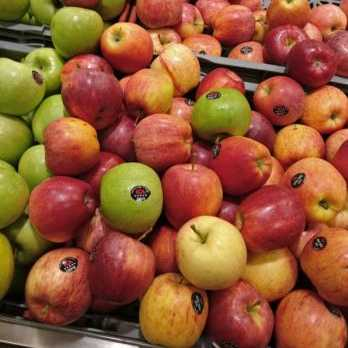
\includegraphics[width=\textwidth]{PaperA/dataset-figure/Royal-Gala-Apple_84_crop.jpg}
			%\vspace{-7mm}
			\caption{Royal Gala}
			\label{subfig:real-image-a}
		\end{subfigure}~
		%\vspace{2pt}
		\begin{subfigure}[t]{0.32\textwidth}
			\centering
			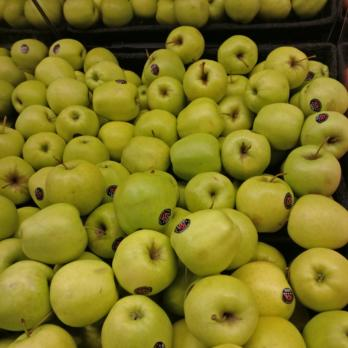
\includegraphics[width=\textwidth]{PaperA/dataset-figure/Golden-Delicious-Apple_7.jpg}
			%\vspace{-7mm}
			\caption{Golden Delicious}
			\label{subfig:real-image-c}
		\end{subfigure}~
		\begin{subfigure}[t]{0.32\textwidth}
			\centering
			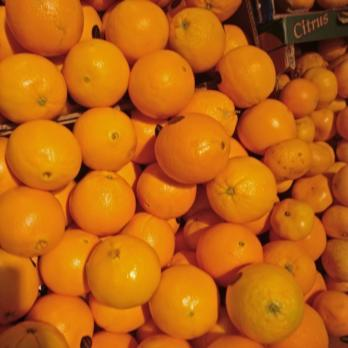
\includegraphics[width=\textwidth]{PaperA/dataset-figure/Orange_025.jpg}
			%\vspace{-7mm}
			\caption{Orange}
			\label{subfig:real-image-f}
		\end{subfigure}~ \\[1mm]
		\begin{subfigure}[t]{0.32\textwidth}
			\centering
			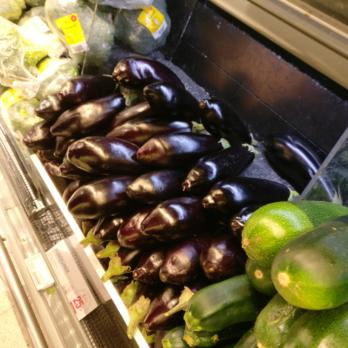
\includegraphics[width=\textwidth]{PaperA/dataset-figure/Aubergine_016.jpg}
			%\vspace{-7mm}
			\caption{Aubergine}
			\label{subfig:real-image-h}
		\end{subfigure}~
		\begin{subfigure}[t]{0.32\textwidth}
			\centering
			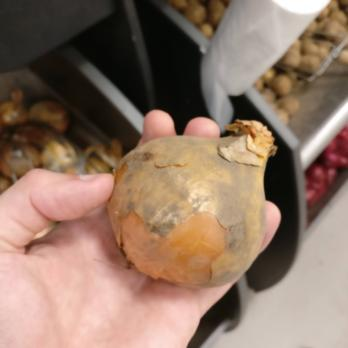
\includegraphics[width=\textwidth]{PaperA/dataset-figure/Yellow-Onion_25.jpg}
			%\vspace{-7mm}
			\caption{Onion}
			\label{subfig:real-image-j}
		\end{subfigure}~
		\begin{subfigure}[t]{0.32\textwidth}
			\centering
			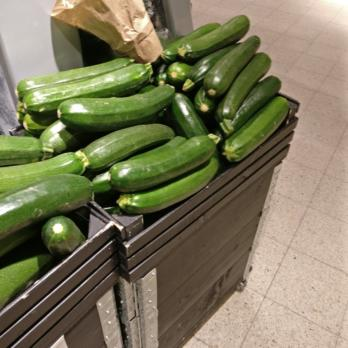
\includegraphics[width=\textwidth]{PaperA/dataset-figure/Zucchini_015.jpg}
			%\vspace{-7mm}
			\caption{Zucchini}
			\label{subfig:real-image-l}
		\end{subfigure}~ \\[1mm]
		\begin{subfigure}[t]{0.32\textwidth}
			\centering
			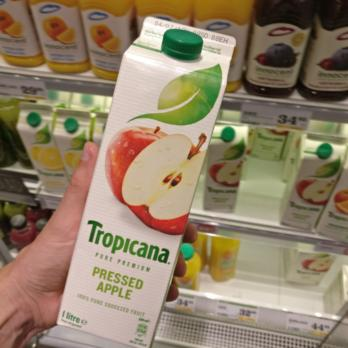
\includegraphics[width=\textwidth]{PaperA/dataset-figure/Tropicana-Apple-Juice_16.jpg}
			%\vspace{-7mm}
			\caption{Apple Juice}
			\label{subfig:real-image-n}
		\end{subfigure}~
		\begin{subfigure}[t]{0.32\textwidth}
			\centering
			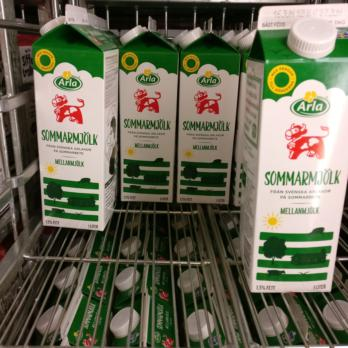
\includegraphics[width=\textwidth]{PaperA/dataset-figure/Arla-Milk-Medium-Fat_17.jpg}
			%\vspace{-7mm}
			\caption{Milk Medium Fat}
			\label{subfig:real-image-q}
		\end{subfigure}~
		\begin{subfigure}[t]{0.32\textwidth}
			\centering
			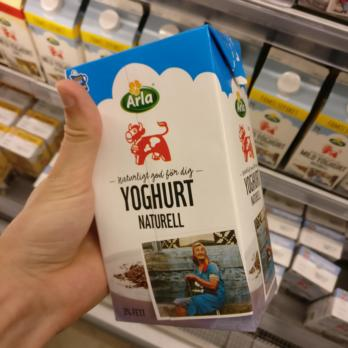
\includegraphics[width=\textwidth]{PaperA/dataset-figure/Arla-Natural-Yoghurt_031.jpg}
			%\vspace{-7mm}
			\caption{Yoghurt Natural}
			\label{subfig:real-image-r}
		\end{subfigure}~ 
		\captionsetup{font=footnotesize}
		\caption{Examples of natural images in our dataset, where each image have been taken inside a grocery store. Image examples of fruits, vegetables and refrigerated products are presented in each row respectively.
		}
		\label{fig:dataset-figure}
	\end{minipage}
	\hspace{10pt}
	%\vspace{-10mm}
	\begin{minipage}[b]{0.47\textwidth}
		%\vspace{-20pt}
		\centering
		\captionsetup{font=scriptsize}
		\begin{subfigure}[t]{0.32\textwidth}
			\centering
			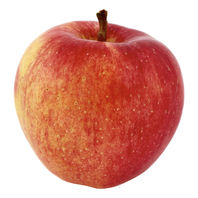
\includegraphics[width=\textwidth]{PaperA/clean-image-figure/Royal-Gala-Apple_Clean.jpg}
			%\vspace{-7mm}
			\caption{Royal Gala}
			\label{subfig:clean-image-a}
		\end{subfigure}~
		\begin{subfigure}[t]{0.32\textwidth}
			\centering
			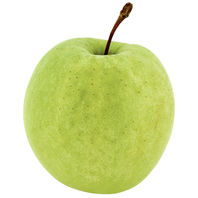
\includegraphics[width=\textwidth]{PaperA/clean-image-figure/Golden-Delicious-Apple_Clean.jpg}
			%\vspace{-7mm}
			\caption{Golden Delicious}
			\label{subfig:clean-image-c}
		\end{subfigure}~
		\begin{subfigure}[t]{0.32\textwidth}
			\centering
			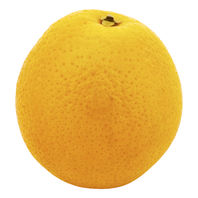
\includegraphics[width=\textwidth]{PaperA/clean-image-figure/Orange_Clean.jpg}
			%\vspace{-7mm}
			\caption{Orange}
			\label{subfig:clean-image-f}
		\end{subfigure}~ \\[1mm]
		\begin{subfigure}[t]{0.32\textwidth}
			\centering
			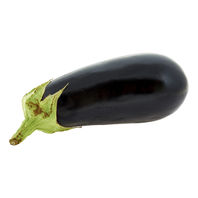
\includegraphics[width=\textwidth]{PaperA/clean-image-figure/Aubergine_Clean.jpg}
			%\vspace{-7mm}
			\caption{Aubergine}
			\label{subfig:clean-image-h}
		\end{subfigure}~
		\begin{subfigure}[t]{0.32\textwidth}
			\centering
			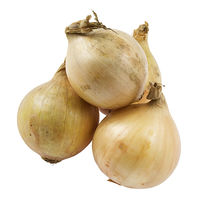
\includegraphics[width=\textwidth]{PaperA/clean-image-figure/Yellow-Onion_Clean.jpg}
			%\vspace{-7mm}
			\caption{Onion}
			\label{subfig:clean-image-j}
		\end{subfigure}~
		\begin{subfigure}[t]{0.32\textwidth}
			\centering
			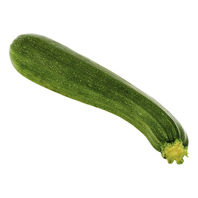
\includegraphics[width=\textwidth]{PaperA/clean-image-figure/Zucchini_Clean.jpg}
			%\vspace{-7mm}
			\caption{Zucchini}
			\label{subfig:clean-image-l}
		\end{subfigure}~ \\[1mm]
		\begin{subfigure}[t]{0.32\textwidth}
			\centering
			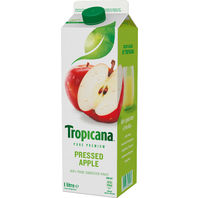
\includegraphics[width=\textwidth]{PaperA/clean-image-figure/Tropicana-Apple-Juice_Clean.jpg}
			%\vspace{-7mm}
			\caption{Apple Juice}
			\label{subfig:clean-image-n}
		\end{subfigure}~
		\begin{subfigure}[t]{0.32\textwidth}
			\centering
			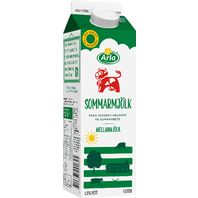
\includegraphics[width=\textwidth]{PaperA/clean-image-figure/Arla-Milk-Medium-Fat_Clean.jpg}
			%\vspace{-7mm}
			\caption{Milk Medium Fat}
			\label{subfig:clean-image-q}
		\end{subfigure}~
		\begin{subfigure}[t]{0.32\textwidth}
			\centering
			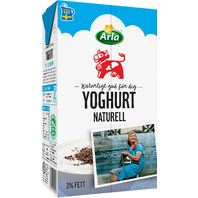
\includegraphics[width=\textwidth]{PaperA/clean-image-figure/Arla-Natural-Yoghurt_Clean.jpg}
			%\vspace{-7mm}
			\caption{Yoghurt Natural}
			\label{subfig:clean-image-r}
		\end{subfigure}~ 
		\captionsetup{font=footnotesize}
		
		\caption{Examples of iconic images downloaded from a grocery shopping website, which corresponds to the target items in the images in Figure \ref{fig:dataset-figure}. \newline }
		\label{fig:clean-image-figure}
	\end{minipage} 
	\vspace{-2mm}
\end{figure}


\section{Related Work}\label{paperA:sec:related_work}

Many popular image datasets have been collected by downloading images from the web \citeA{paperA:deng2009imagenet, paperA:Everingham2010pascal, paperA:Gebru2017FineGrainedCD,  paperA:griffin2007caltech256, paperA:Krizhevsky2009cifar100, paperA:Lin2014MicrosoftCoco, paperA:song2016deep, paperA:welinder2010birds, paperA:xiao2010sundatabase}. 
If the dataset contains a large amount of images, it is convenient to make use of crowdsourcing to get annotations for recognition tasks \citeA{paperA:deng2009imagenet, paperA:Krizhevsky2009cifar100, paperA:liu2015faceattributes}. For some datasets, the crowdsourcers are also asked to put bounding boxes around the object to be labeled for object detection tasks \citeA{paperA:Everingham2010pascal, paperA:Gebru2017FineGrainedCD, paperA:welinder2010birds}. In \citeA{paperA:griffin2007caltech256} and \citeA{paperA:Krizhevsky2009cifar100}, the target objects are usually centered and takes up most content of the image itself. Another significant characteristic is that web images usually are biased in the sense that they have been taken with the object focus in mind; they have good lighting settings and are typically clean from occlusions, since the collectors have used general search words for the object classes, e.g. \textit{car}, \textit{horse}, or \textit{apple}.

Some datasets include additional information about the images beyond the single class label, e.g. text descriptions of what is present in the image and bounding boxes around objects. These datasets can be used in several different computer vision tasks, such as image classification, object detection, and image segmentation. Structured labeling is another important property of a dataset, which provides flexibility when classifying images. In  \citeA{paperA:Gebru2017FineGrainedCD, paperA:Lin2014MicrosoftCoco}, all of these features exist and moreover they include reference images to each object class, which in \citeA{paperA:Lin2014MicrosoftCoco} is used for labeling multiple  categories present in images, while in \citeA{paperA:Gebru2017FineGrainedCD} these images are used for fine-grained recognition. 
Our dataset includes a reference image, i.e. the iconic image, and a product description for every class, and we have also labeled the grocery items in a structured manner.

Other image datasets of fruits and vegetables for classification purposes are the FIDS30 database \citeA{paperA:marko2013fids30} and the dataset in \citeA{paperA:muresan2017fruit}. The images in FIDS30 were downloaded from the web and contain background noise as well as single or multiple instances of the object. In \citeA{paperA:muresan2017fruit}, all pixels belonging to the object are extracted from the original image, such that all images have white backgrounds with the same brightness condition. There also exist datasets for detecting fruits in orchards for robotic harvesting purposes, which are very challenging since the images contain plenty of background and various lighting conditions, and the targeted fruits are often occluded or of the same color as the background \citeA{paperA:bargoti2017deepfruitdetection, paperA:sa2016deepfruits}.

Another dataset that is highly relevant to our application need is presented in  \citeA{paperA:waltner2015mango}. They collected a dataset for training and evaluating the image classifier by extracting images from video recordings of 23 main classes, which are subdivided into 98 classes, of raw grocery items (fruits and vegetables) in different grocery stores. Using this dataset, a mobile application was developed to recognize food products in grocery store environments, which provides the user with details and health recommendations about the item along with other proposals of similar food items. For each class, there exists a product description with nutrition values to assist the user in shopping scenarios. The main difference between this work and our dataset is firstly the clean iconic images (visual labels) for each class in our dataset, and secondly that we have also collected images of refrigerated items, such as dairy and juice containers, where visual information is required to distinguish between the products.   
